% Datapath del FIR RRC en el tiempo, forma directa, versión serial.
% Compilar: ver doc/diagramas/compilar.sh
\documentclass[tikz,border=8pt]{standalone}
\usepackage[T1]{fontenc}
\usepackage{lmodern}
\usepackage{amsmath}
\renewcommand{\familydefault}{\sfdefault}
\usetikzlibrary{arrows.meta,calc,positioning,backgrounds}

\begin{document}
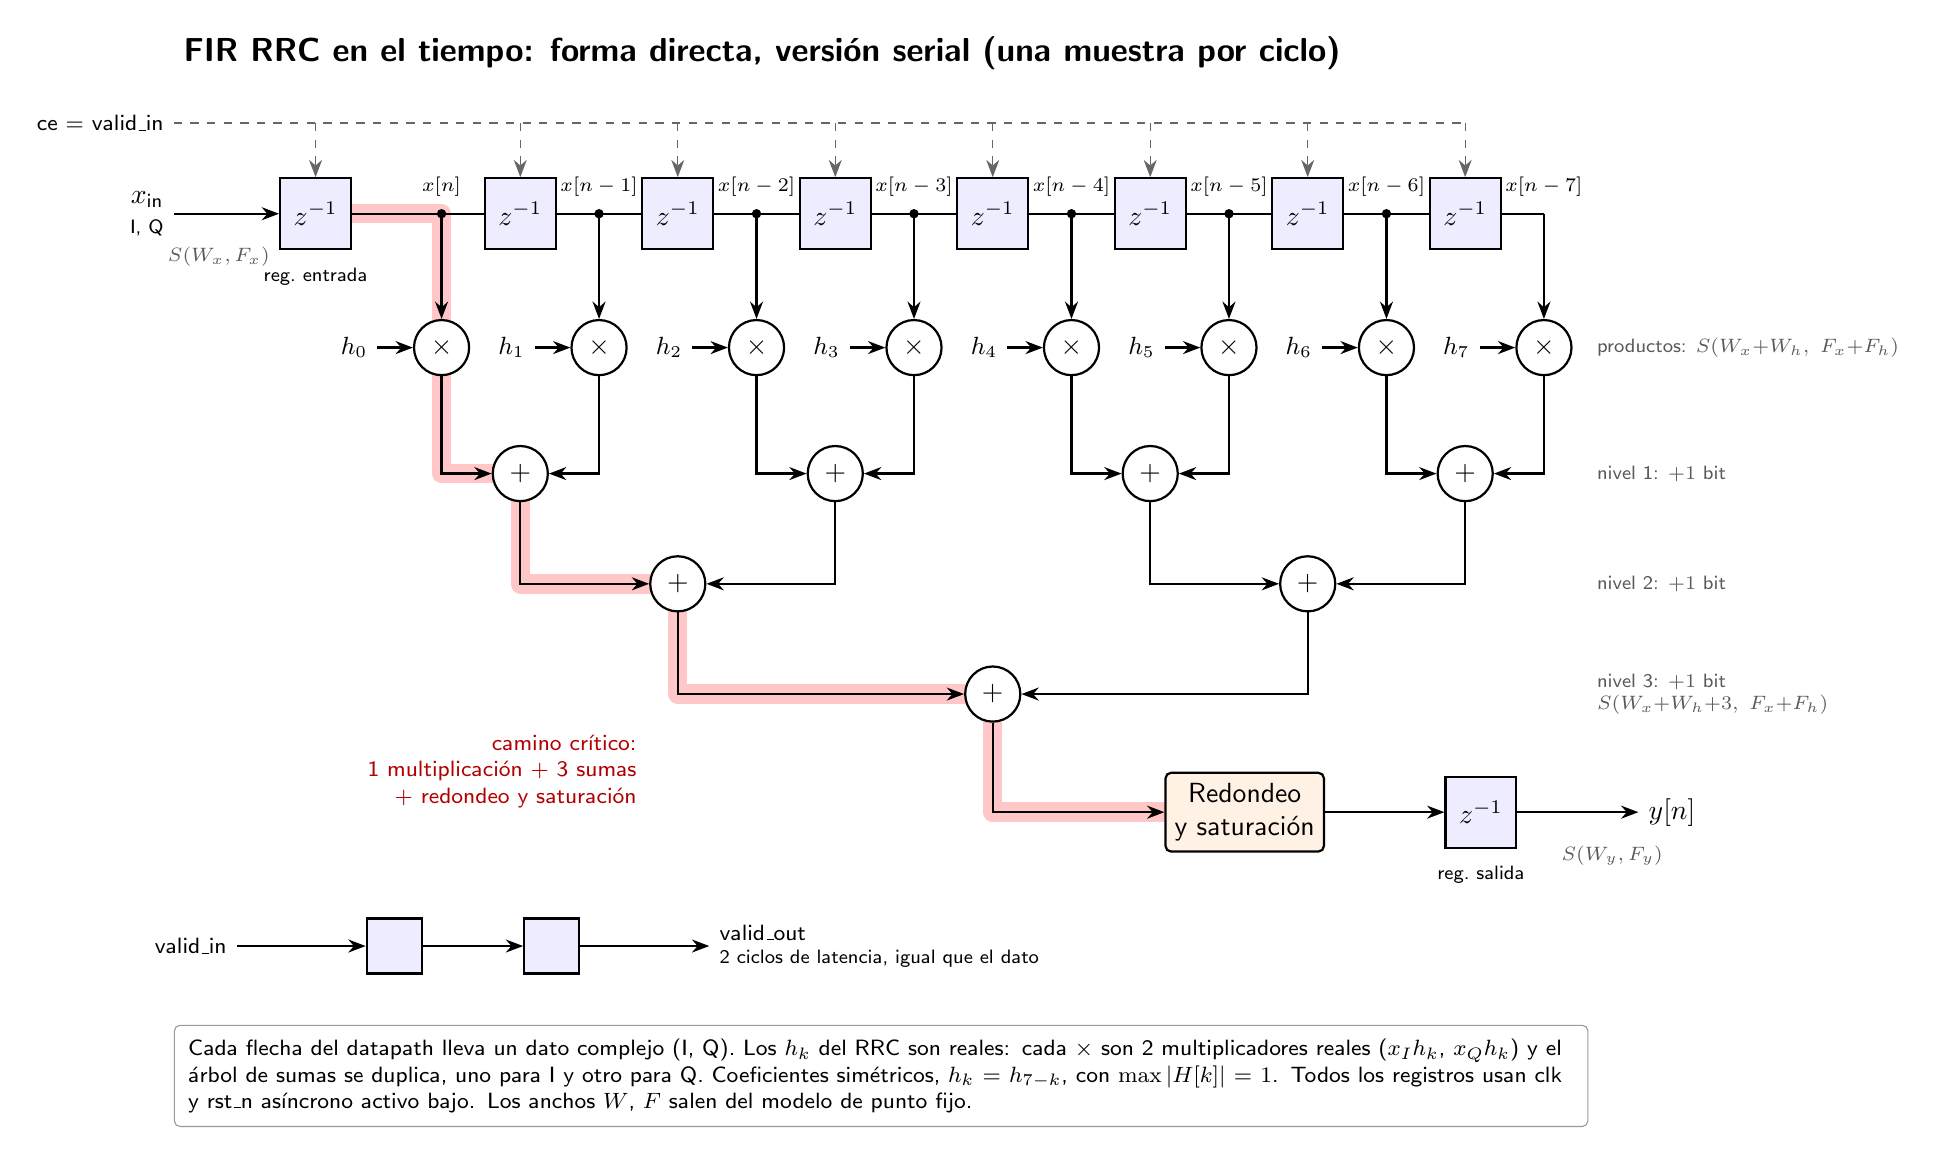
\begin{tikzpicture}[
  >={Stealth[length=2.2mm]},
  reg/.style={draw,thick,minimum width=9mm,minimum height=9mm,fill=blue!7},
  op/.style={draw,thick,circle,minimum size=7mm,inner sep=0pt,fill=white},
  bloque/.style={draw,thick,rounded corners=2pt,minimum height=10mm,align=center,fill=orange!10},
  dato/.style={->,thick},
  fmt/.style={font=\scriptsize,text=black!65,anchor=west},
  etiq/.style={font=\scriptsize},
]

% ---------------- línea de retardo ----------------
\node[reg] (rin) at (-1.6,0) {$z^{-1}$};
\node[etiq,below=1mm of rin] {reg.\ entrada};
\draw[dato] (-3.4,0) node[left,align=right]{$x_{\text{in}}$\\[-1pt]{\scriptsize I, Q}} -- (rin);
\node[fmt] at (-3.6,-0.55) {$S(W_x,F_x)$};

\foreach \k in {0,...,7} {\coordinate (t\k) at (2*\k,0);}
\draw[thick] (rin) -- (t0);
\foreach \k [evaluate=\k as \s using int(\k+1)] in {0,...,6} {
  \node[reg] (z\k) at (2*\k+1,0) {$z^{-1}$};
  \draw[thick] (t\k) -- (z\k);
  \draw[thick] (z\k) -- (t\s);
}
\node[etiq,above=1mm] at (t0) {$x[n]$};
\foreach \k in {1,...,7} {\node[etiq,above=1mm] at (t\k) {$x[n-\k]$};}

% habilitación de corrimiento
\draw[dashed,thick,black!60] (-3.4,1.15) node[left,black,font=\footnotesize]{ce $=$ valid\_in} -- (13,1.15);
\foreach \r in {rin,z0,z1,z2,z3,z4,z5,z6} {
  \draw[->,dashed,black!60] (\r.north |- 0,1.15) -- (\r.north);
}

% ---------------- multiplicadores ----------------
\foreach \k in {0,...,7} {
  \node[op] (m\k) at (2*\k,-1.7) {$\times$};
  \draw[dato] (t\k) -- (m\k);
  \draw[<-,thick] (m\k.west) -- ++(-0.45,0) node[left,font=\small]{$h_{\k}$};
}
\foreach \k in {0,...,6} {\fill (t\k) circle (1.7pt);}

% ---------------- árbol de sumas ----------------
\node[op] (a0) at (1,-3.3)  {$+$};
\node[op] (a1) at (5,-3.3)  {$+$};
\node[op] (a2) at (9,-3.3)  {$+$};
\node[op] (a3) at (13,-3.3) {$+$};
\node[op] (b0) at (3,-4.7)  {$+$};
\node[op] (b1) at (11,-4.7) {$+$};
\node[op] (c0) at (7,-6.1)  {$+$};
\draw[dato] (m0) |- (a0);  \draw[dato] (m1) |- (a0);
\draw[dato] (m2) |- (a1);  \draw[dato] (m3) |- (a1);
\draw[dato] (m4) |- (a2);  \draw[dato] (m5) |- (a2);
\draw[dato] (m6) |- (a3);  \draw[dato] (m7) |- (a3);
\draw[dato] (a0) |- (b0);  \draw[dato] (a1) |- (b0);
\draw[dato] (a2) |- (b1);  \draw[dato] (a3) |- (b1);
\draw[dato] (b0) |- (c0);  \draw[dato] (b1) |- (c0);

% ---------------- salida ----------------
\node[bloque] (rs) at (10.2,-7.6) {Redondeo\\ y saturación};
\node[reg] (rout) at (13.2,-7.6) {$z^{-1}$};
\node[etiq,below=1mm of rout] {reg.\ salida};
\draw[dato] (c0) |- (rs);
\draw[dato] (rs) -- (rout);
\draw[dato] (rout) -- (15.2,-7.6) node[right]{$y[n]$};
\node[fmt] at (14.1,-8.15) {$S(W_y,F_y)$};

% formatos a la derecha
\node[fmt] at (14.55,-1.7) {productos: $S(W_x{+}W_h,\ F_x{+}F_h)$};
\node[fmt] at (14.55,-3.3) {nivel 1: $+1$ bit};
\node[fmt] at (14.55,-4.7) {nivel 2: $+1$ bit};
\node[fmt,align=left] at (14.55,-6.1) {nivel 3: $+1$ bit\\ $S(W_x{+}W_h{+}3,\ F_x{+}F_h)$};

% ---------------- camino crítico ----------------
\begin{scope}[on background layer]
  \draw[line width=7pt,red!22,line cap=round,line join=round]
    (rin.east) -- (t0) -- (m0.center) |- (a0.center) |- (b0.center)
    |- (c0.center) |- (rs.west);
\end{scope}
\node[font=\footnotesize,text=red!70!black,align=right,anchor=north east] at (2.6,-6.5)
  {camino crítico:\\ 1 multiplicación + 3 sumas\\ + redondeo y saturación};

% ---------------- control ----------------
\node[reg,minimum width=7mm,minimum height=7mm] (v1) at (-0.6,-9.3) {};
\node[reg,minimum width=7mm,minimum height=7mm] (v2) at (1.4,-9.3) {};
\draw[dato] (-2.6,-9.3) node[left,font=\footnotesize]{valid\_in} -- (v1);
\draw[dato] (v1) -- (v2);
\draw[dato] (v2) -- (3.4,-9.3) node[right,font=\footnotesize,align=left]{valid\_out\\[-1pt]\scriptsize 2 ciclos de latencia, igual que el dato};

% ---------------- notas ----------------
\node[draw=black!40,rounded corners=2pt,font=\footnotesize,align=left,anchor=north west,
      text width=17.6cm,inner sep=5pt] at (-3.4,-10.3) {%
  Cada flecha del datapath lleva un dato complejo (I, Q). Los $h_k$ del RRC son reales: cada $\times$ son
  2 multiplicadores reales ($x_I h_k$, $x_Q h_k$) y el árbol de sumas se duplica, uno para I y otro para Q.
  Coeficientes simétricos, $h_k = h_{7-k}$, con $\max|H[k]| = 1$.
  Todos los registros usan clk y rst\_n asíncrono activo bajo. Los anchos $W$, $F$ salen del modelo de punto fijo.};

\node[font=\large\bfseries,anchor=south west] at (-3.4,1.7)
  {FIR RRC en el tiempo: forma directa, versión serial (una muestra por ciclo)};
\end{tikzpicture}
\end{document}
